\newcommand{\institut}{Institut f\"ur Telekommunikationssysteme}
\newcommand{\fachgebiet}{Nachrichten\"ubertragung}
\newcommand{\veranstaltung}{Praktikum Nachrichten\"ubertragung}
\newcommand{\pdfautor}{Dirk Babendererde (321 836), Thomas Kapa (325 219)}
\newcommand{\autor}{Dirk Babendererde (321 836)\\ Thomas Kapa (325 219)}
\newcommand{\gruppe}{Gruppe:}
\newcommand{\betreuer}{Betreuer: Lieven Lange}


\newcommand{\pdftitle}{Nachrichten\"ubertragung\ Praktikum\ 02}
\newcommand{\prototitle}{Praktikum 02 \\ Statistische Nachrichtentheorie}

\input{../../packages/tu_header_8}


% \lstlistoflistings
\definecolor{darkgray}{rgb}{0.95,0.95,0.95}
\definecolor{darkolivegreen}{HTML}{01a801}
\definecolor{functionsBlue}{HTML}{32b9b9}
\definecolor{variableRed}{rgb}{1,0,0}
\definecolor{stringBrown}{HTML}{bc8e8e} % f geht nicht

\lstset{
        %\lstset{extendedchars=true} % Umlaute an der richtigen stelle und nicht am Anfang ausgeben
        %basicstyle=\footnotesize\ttfamily,
        basicstyle=\small,
        %
        inputencoding=utf8,
        %
        tabsize=4,
        showspaces=false,
        showtabs=false,
        showstringspaces=true, % no special string spaces
        %
        backgroundcolor=\color{darkgray}, % background
        stringstyle=\color{stringBrown}\fseries, % Strings
        keywordstyle=\color{functionsBlue}\bfseries, % keywords Blau
        identifierstyle=\color{variableRed}, % variablen
        commentstyle=\color{darkolivegreen}, %  comments
        %
        breaklines=true,
        %
        numbers=left,
        numberstyle=\tiny,
        stepnumber=1,
        numbersep=7pt,
        %
        frame=single,
        columns=flexible,
        %
        xleftmargin=-2cm,
        xrightmargin=-1.5cm,
        %
        language=Matlab,
}
% enables UTF-8 in source code: (dirty, dirty hack)
\lstset{literate=
    %Deutsch
    {ä}{{\"a}}1 {ö}{{\"o}}1 {ü}{{\"u}}1 {Ä}{{\"A}}1 {Ö}
    {{\"O}}1 {Ü}{{\"U}}1 {ß}{\ss}1
    %Türkisch
    {â}{{\^{a}}}1 {Â}{{\^{A}}}1 {ç}{{\c{c}}}1 {Ç}{{\c{C}}}1 {ğ}{{\u{g}}}1 {Ğ}{{\u{G}}}1 {ı}{{\i}}1 {İ}{{\.{I}}}1 {ö}{{\"o}}1 {Ö}{{\"O}}1 {ş}{{\c{s}}}1
    {Ş}{{\c{S}}}1 {ü}{{\"u}}1 {Ü}{{\"U}}1
    %Polish
    {ą}{{\k{a}}}1 {ć}{{\'c}}1 {ę}{{\k{e}}}1 {ł}{{\l{}}}1 {ń}{{\'n}}1 {ó}{{\'o}}1 {ś}{{\'s}}1 {ż}{{\.z}}1 {ź}{{\'z}}1 {Ą}{{\k{A}}}1 {Ć}{{\'C}}1
    {Ę}{{\k{E}}}1 {Ł}{{\L{}}}1 {Ń}{{\'N}}1 {Ó}{{\'O}}1 {Ś}{{\'S}}1 {Ż}{{\.Z}}1 {Ź}{{\'Z}}1
    %Spanish
    {á}{{\'a}}1 {é}{{\'e}}1 {í}{{\'i}}1 {ó}{{\'o}}1 {ú}{{\'u}}1 {ñ}{{\~n}}1
}

%     \lstinputlisting{./praktikum6.sce}



%---------------------------------------------------------------------
%---------------------------------------------------------------------
%---------------------------------------------------------------------

\section{Vorbereitungsaufgaben}

    \begin{quote}
    Berechnet die Varianz von gleichverteiltem weißem Rauschen N mit der
    Verteilungsdichtefunktion $p_{N}(n)=\frac{1}{2A}\sqcap_{2A}(n)$. Zunächst
    berechnet man den Mittelwert und die Leistung und kann daraus die Varianz
    bestimmen.
    \begin{equation*}
     \begin{split}
     \mu &= \int_{-\infty}^{+\infty} n \frac{1}{2A} \sqcap_{2A} (n) \mathrm dn\\
     &= \int_{-A}^{+A} n \frac{1}{2A} \mathrm dn\\
     &= \left[ \frac{1}{2A} \frac{1}{2} n^2 \right]_{-A}^{+A}\\
     &= \frac{1}{4A} (A^2-(-A)^2)\\
     &= 0
     \end{split}
    \end{equation*}
    
    \begin{equation*}
     \begin{split}
     P &= \int_{-\infty}^{+\infty} n^2 \frac{1}{2A} \sqcap_{2A} (n) \mathrm dn\\
     &= \int_{-A}^{+A} n^2 \frac{1}{2A} \mathrm dn\\
     &= \left[ \frac{1}{2A} \frac{1}{3} n^3 \right]_{-A}^{+A}\\
     &= \frac{1}{6A} (A^3-(-A)^3)\\
            &= \frac{2A^3}{6A} = \frac{1}{3} A^2\\
     \end{split}
    \end{equation*}
    
    \begin{equation*}
     \begin{split}
     \sigma^2 &= P - \mu^2\\
     &= \frac{1}{3} A^2 - 0 = \frac{1}{3} A^2
     \end{split}
    \end{equation*}
\end{quote}



\section{Vorbereitungsaufgaben}
\begin{quote}
    \hspace{-2em}
    \subsection{Varianz von gleichverteiltem weißem Rauschen}
    Berechnet die Varianz von gleichverteiltem weißem Rauschen N mit der Verteilungsdichtefunktion.\\
    
     \begin{equation*}
    	\begin{split}
    	    \mu_{N}&=E[N]=\int\limits_{-A}^{A} n \cdot \frac{1}{2A} \,dn=0 \\
    		\sigma_{N}^2&=E[(N-\mu_{N})^2]=\int\limits_{-\infty}^{\infty} (n-\mu)^2
    		\cdot p_{u}\,(n) \,dn=\frac{1}{3}A^2
    	\end{split}
     \end{equation*}
    
    
    \begin{quote}
    
    \end{quote}
      
\end{quote}

%--------------------------------------------------------------------
%--------------------------------------------------------------------


\section{Simulation eines Zufallsexperiments mit MatLab: Würfelexperiment}
\begin{quote}
    
    
    \subsection{Labordurchführung}
    \begin{quote}
        
        Wir untersuchen die Eigenschaften von Zufallsexperimenten anhand des Würfelexperiments.
        Hierzu Simulieren wir den sehr häufigen Wurf verschiedenen Anzahl an Würfeln mit von Matlab bereitgestellten
        Zufallsfunktion.\\
        Die Ergebnisse lassen wir uns als normierte (durch die Anzahl der Würfe geteilte) Häufigkeitsverteilung ausgeben und
        vergleichen sie später noch mit mit der theoretischen Verteilungsdichtefunktion.\\
        Nach dem gesetz der großen Zahlen erwarten wir, dass sich die normierte Häufigkeitsverteilung der
        Verteilungsdichtefunktion annähert.
        
    \end{quote}
    
    
    
    
    
    \subsection{Auswertung}
    \begin{quote}
        
        \subsubsection{Fairer Würfel?}
        Der MatLab-Code aus der Vorgabedatei Aufgabe1.m simuliert die 10.000-fache Durchführung eines Würfelexperiments. Ergänzt
        den Code, so dass aus dem einfachen Histogramm die geschätzte pdf des Experiments wird. Handelt es sich um einen fairen
        Würfel?
        
        \begin{quote}
        
            
            Bei einem fairen Würfel erwarten wir, dass bei relativ häufigem Wurf die Augenzahlen gleichhäufig fallen. Die
            normierte Häufigkeitsverteilung sollte also eine Gleichverteilung zeigen; jede Augenzahl müsste die Wahrscheinlichkeit
            $\frac{1}{6}$ haben.\\
            
            
            \begin{figure}[H]
            \centering
                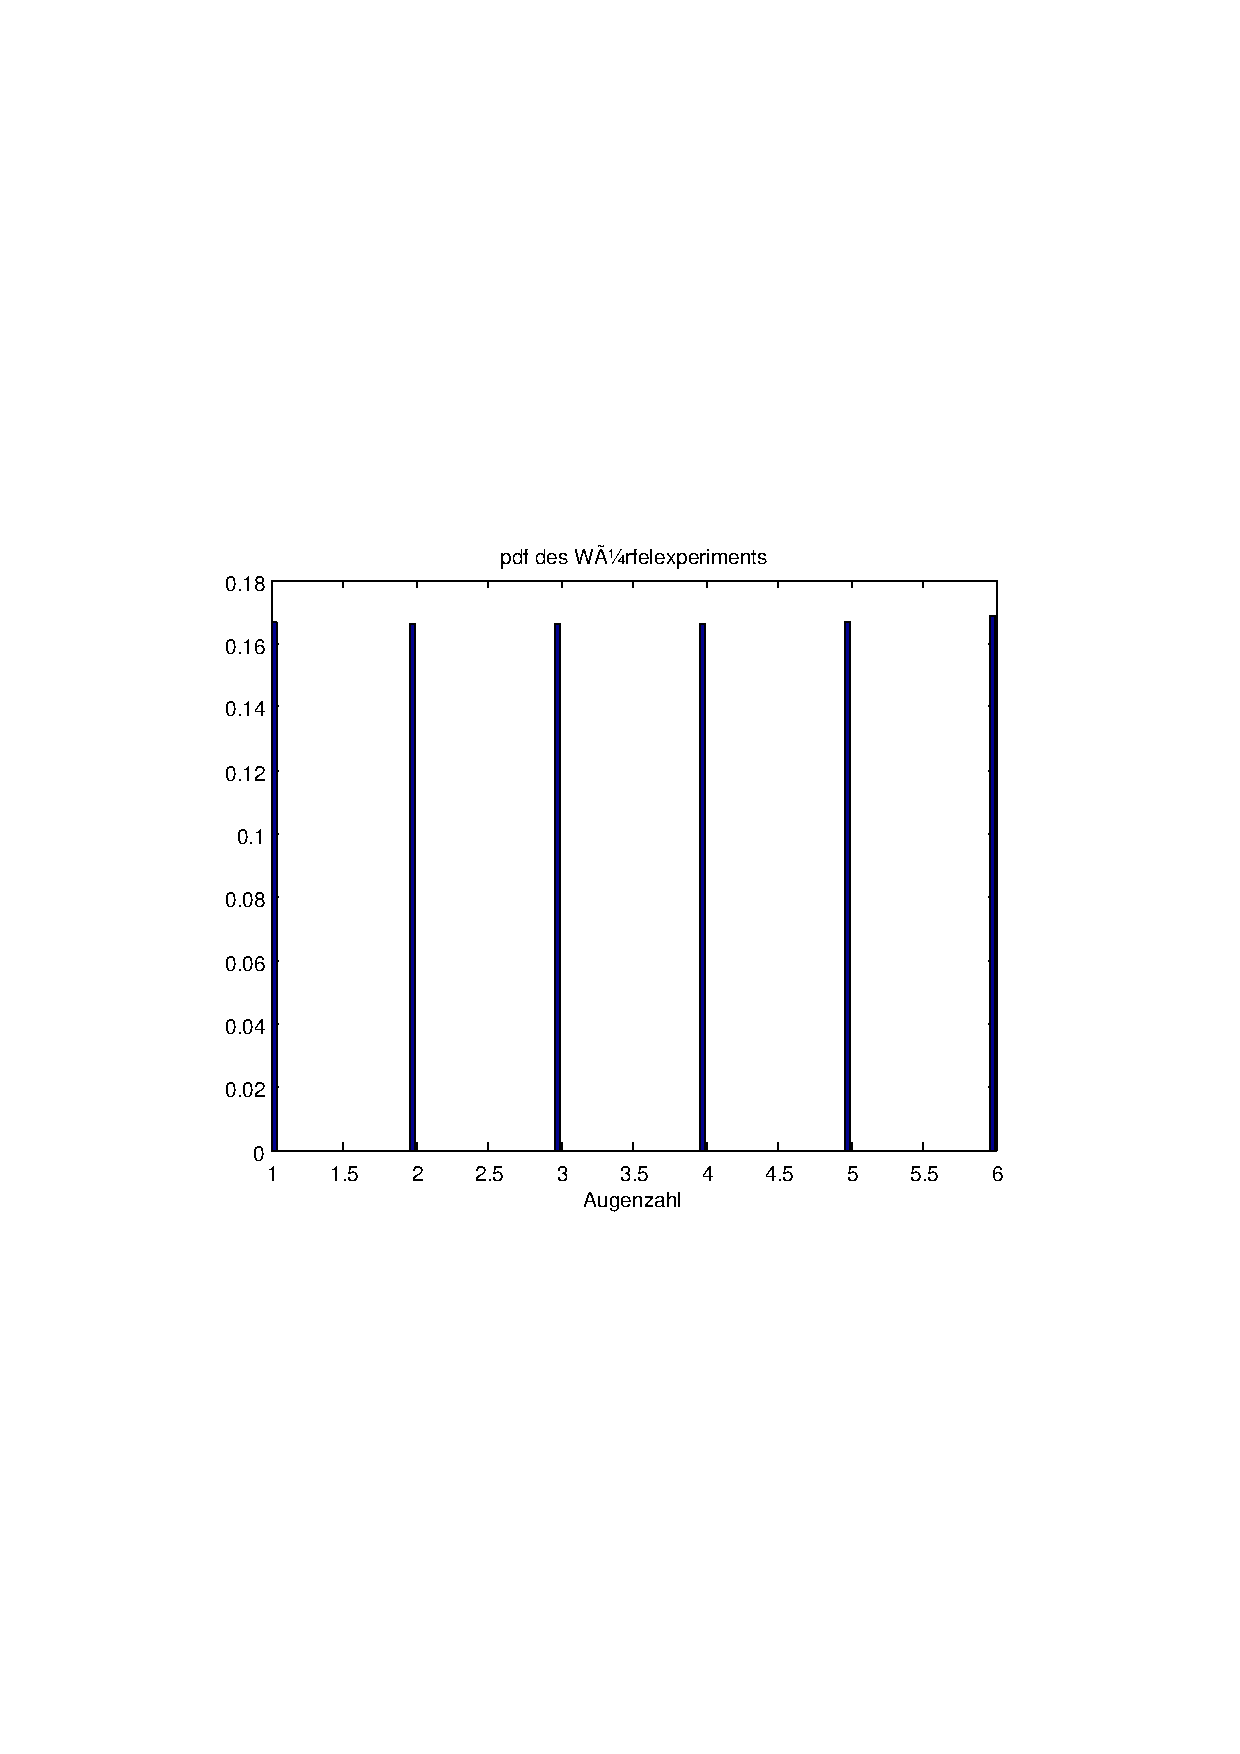
\includegraphics[scale=0.7, trim = 20mm 80mm 20mm 90mm, clip]{Bilder/fairer_wuerfel}
                    \caption{Häufigkeitsverteilung}
                    \label{fig:fairer_wuerfel}
            \end{figure}
            
            Wie in der Häufigkeitsverteilung \ref{fig:fairer_wuerfel} erkennbar ist, ähnelt sie stark einer Gleichverteilung.
            Auch die Häufigkeit ist bei allen sech Seiten des Würfels sehr nahe $\frac{1}{6}$. Somit haben anscheinend alle Seiten
            des Würfels die Gleiche Wahrscheinlichkeit.
            Der Würfel ist also fair.
            
            \vspace{3em}
            \lstinputlisting[
                caption={Matlab-script},
                label=lst:Matlab]
                {./Matlab/Aufgabe1_1.m}
                
        \end{quote}
        
        
        \subsubsection{Summe aus Zwei Würfeln}
        Simuliert nun ein Experiment mit zwei Würfeln, bei dem nach jedem Wurf die Summe der Augenzahlen gebildet wird. Bestimmt
        auch für diesen Fall die pdf.
        
        \begin{quote}
            
            Die Logische Erwartung hierfür ist, dass es für das Ereignis 7 am meisten Kombiinationsmäglichkeiten
            der beiden Würfel gibt und es somit das wahrscheinlichste Ereignis ist. Die Wahrscheinlichkeiten nehmen dann
            in beide Richtungen linear ab, da die Kombinationsmöglichkeiten linear abnehmen.\\
            Die Theorie besagt hierzu, dass die Verteilungsdichtefunktion des Experiments mit zwei Würfeln (ein
            Dreieck) die Faltung zweier Verteilungsdichtefunktionen des selben Experiments mit nur einem Würfel (Rechteck) ist.
            
            \begin{figure}[H]
            \centering
                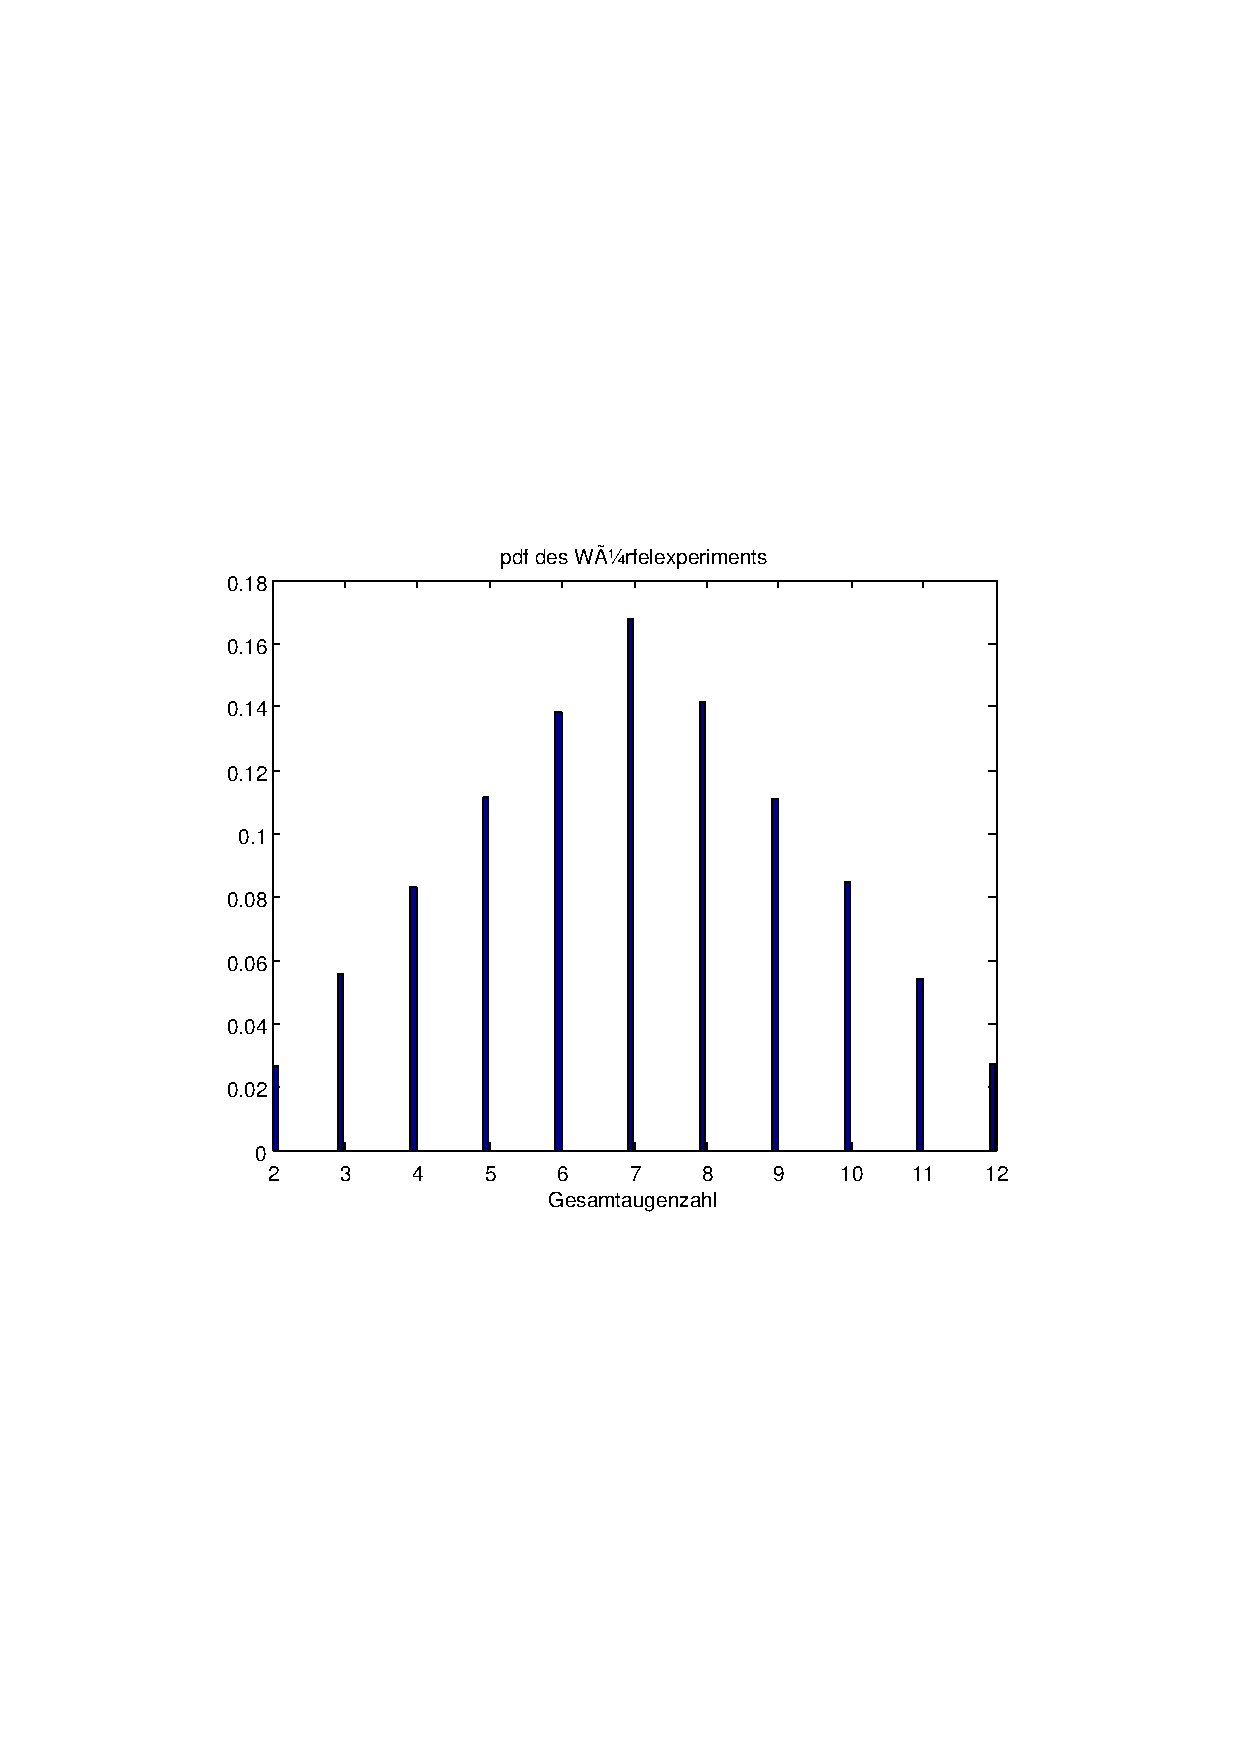
\includegraphics[scale=0.7, trim = 20mm 80mm 20mm 90mm, clip]{Bilder/A1_2}
                    \caption{Häufigkeitsverteilung}
                    \label{fig:A1_2}
            \end{figure}
            
            Auch diese Verteilungsdichtefunktion ist wie erwartet, ein Dreieck. Die nur extrem geringen Abweichungen der
            Simulation gegenüber der Theorie sind mit der sehr häufigen Durchführung und damit dem auftreten des Gesetzes der
            großen Zahlen erklärbar.
            
            \vspace{3em}
            \lstinputlisting[
                caption={Matlab-script},
                label=lst:Matlab]
                {./Matlab/Aufgabe1_2.m}
                
        \end{quote}
        
        
        
        \subsubsection{Zentraler Grenzwertsatz der Statistik}
        Laut zentralem Grenzwertsatz der Statistik, ergibt sich bei Aufsummierung von Zufallsvariablen mit
        weitgehend beliebigen Verteilungsfunktion als Ergebnis eine Zufallsvariable mit Gaußverteilung.
        Dieser Zusammenhang wird in Abbildung 1 des Aufgabenblattes verdeutlicht. Versucht den Grenzwertsatz nachzuvollziehen,
        indem ihr schrittweise erst 10 dann 100 und schließlich 1000 Realisierungen des Würfelexperiments additiv überlagert und die pdfs bestimmt.
        
        
        \begin{center}
        \begin{tabular}{ll}
        
        \hspace{-5cm}
            \begin{minipage}{0.6\textwidth}
                
                \begin{figure}[H]
                    \label{fig:funktion0alpha}
                    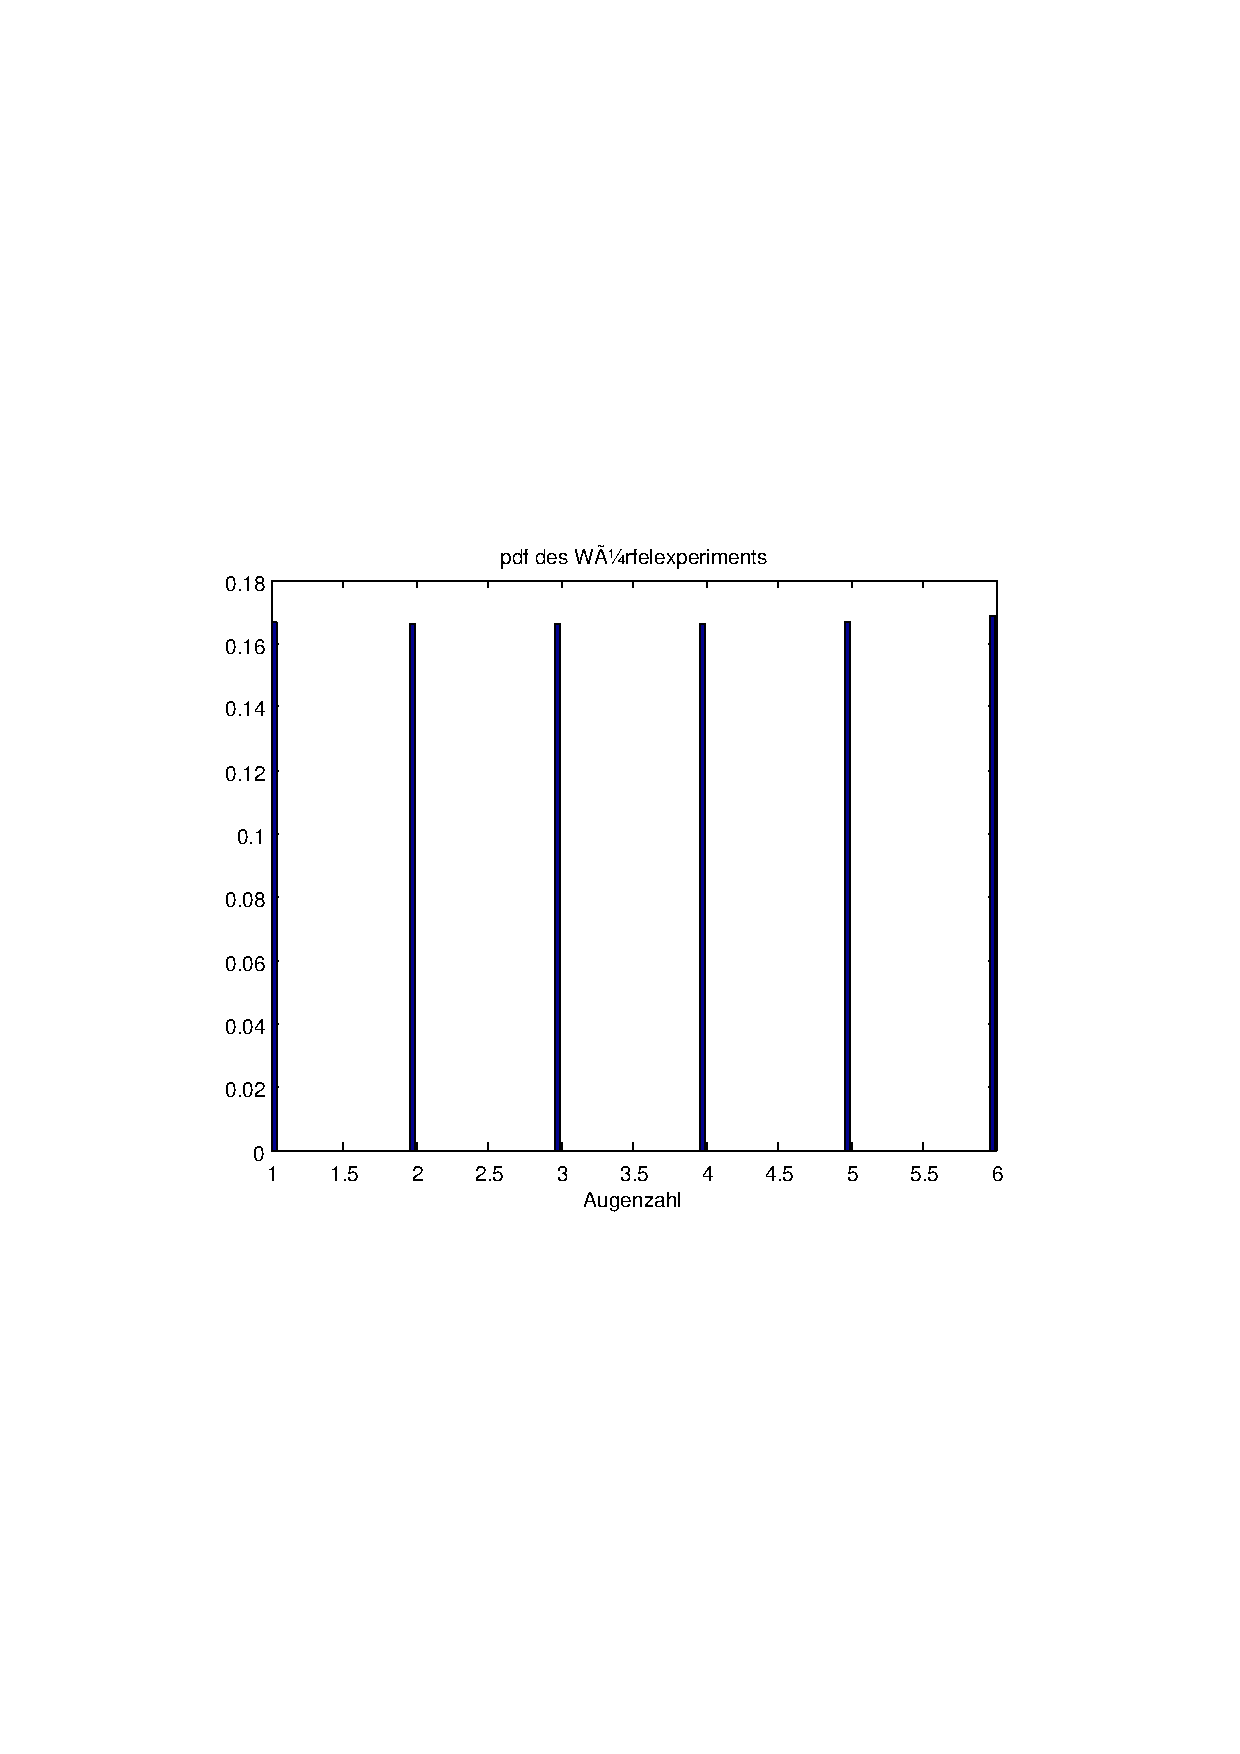
\includegraphics[scale=0.7, trim = 20mm 80mm 20mm 90mm, clip]{Bilder/fairer_wuerfel}
                    \caption{Häufigkeitsverteilung: ein Würfel}
                \end{figure}
        
            \end{minipage}
        
            \begin{minipage}{0.6\textwidth}
                \begin{figure}[H]
                    \label{fig:pico_funktion0alpha}
                    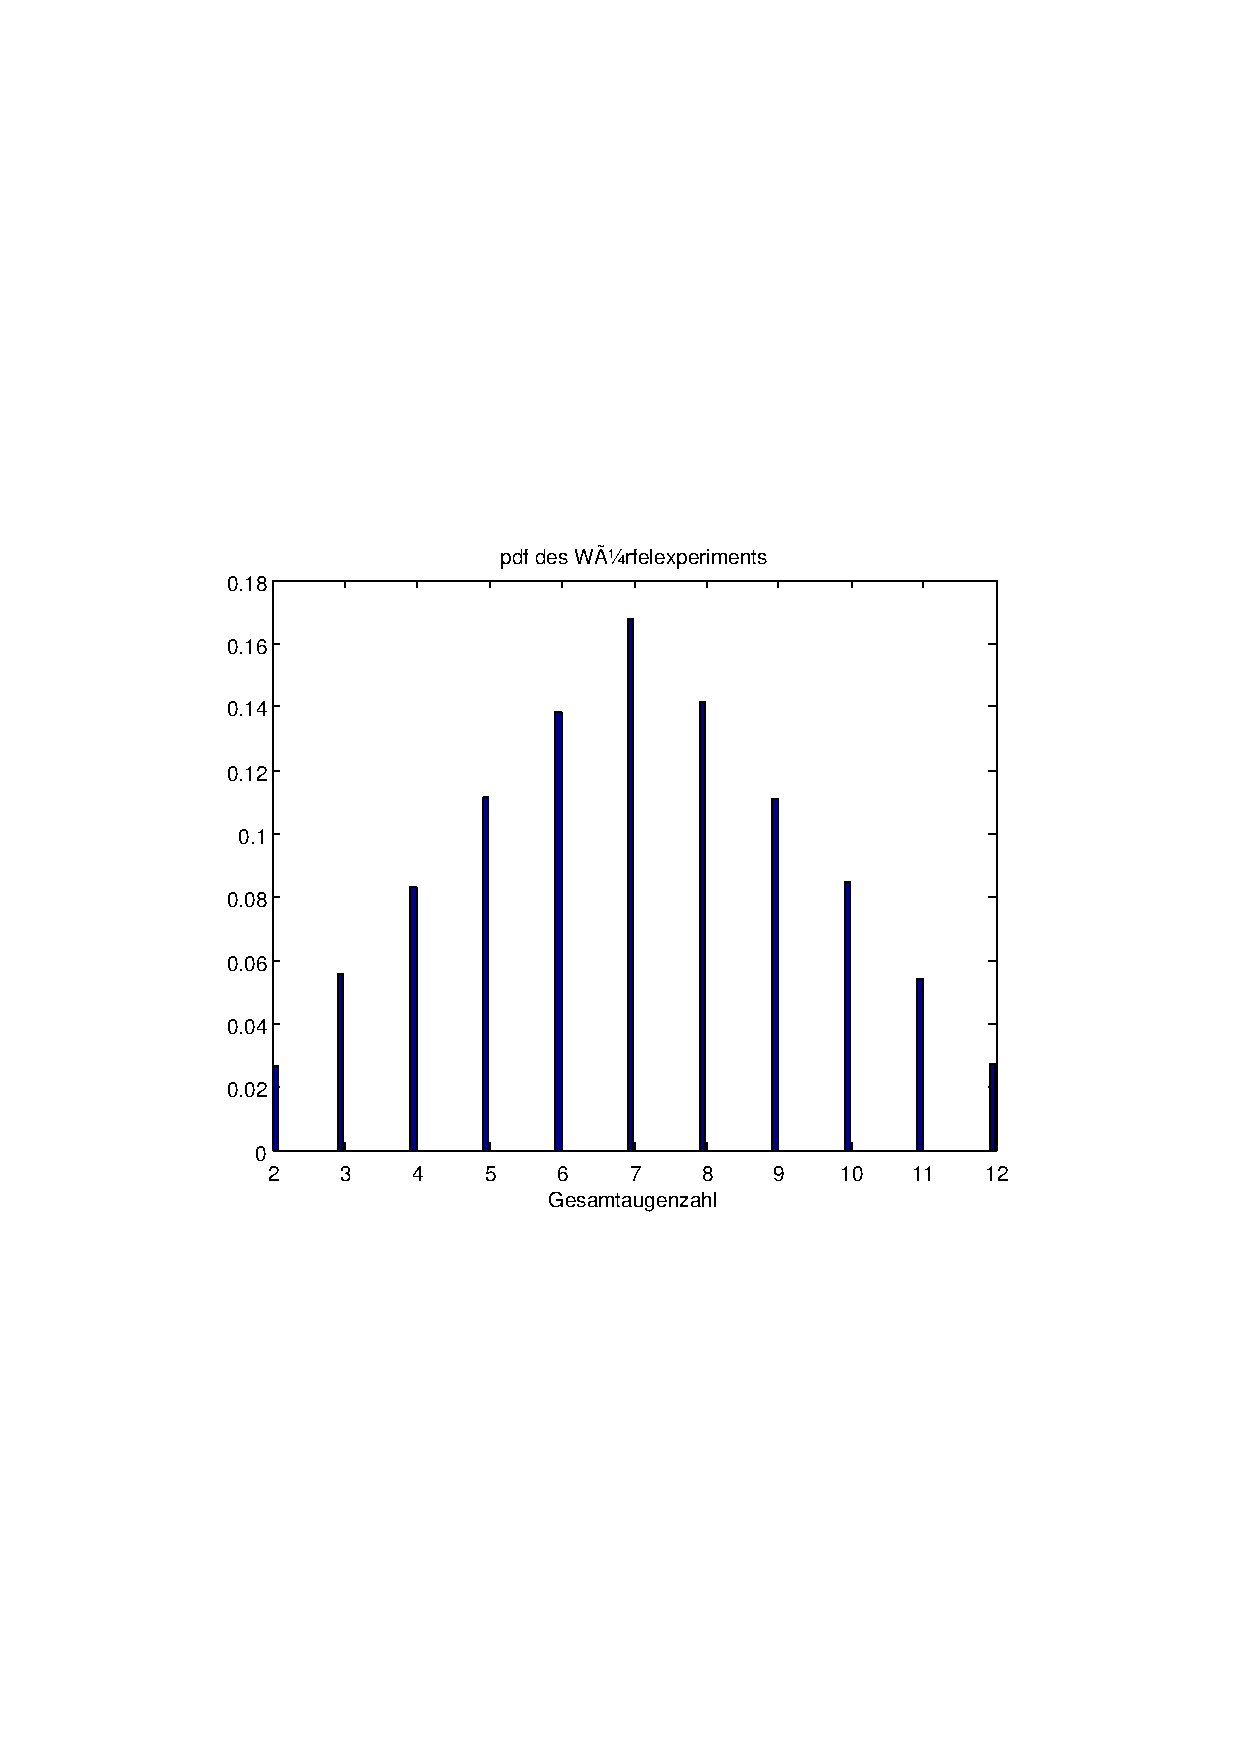
\includegraphics[scale=0.7, trim = 20mm 80mm 20mm 90mm, clip]{Bilder/A1_2}
                    \caption{Häufigkeitsverteilung: zwei Würfel}
                \end{figure}
        
            \end{minipage}
        
        \end{tabular}
        \end{center}

        \begin{center}
        \begin{tabular}{ll}
        
        \hspace{-5cm}
            \begin{minipage}{0.6\textwidth}
                
                \begin{figure}[H]
                    \label{fig:funktion0alpha}
                    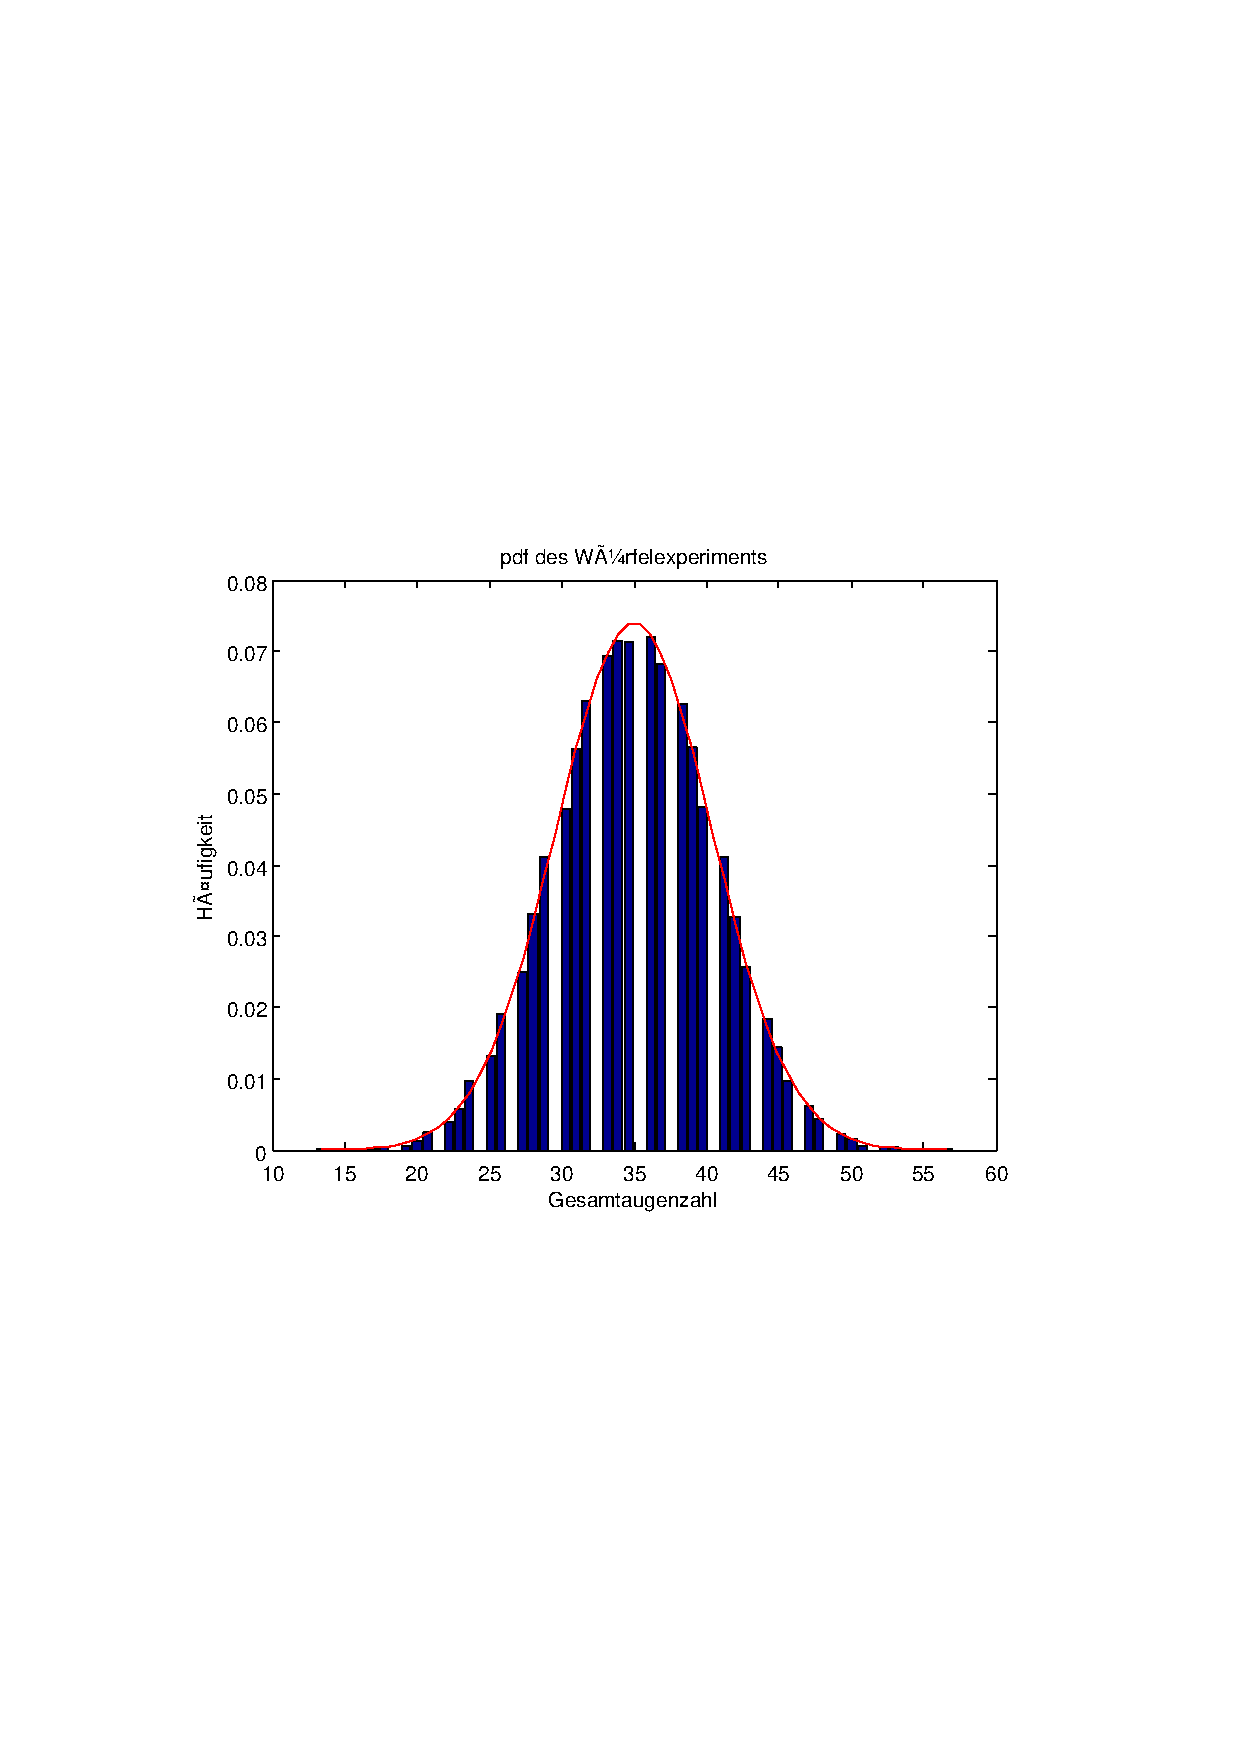
\includegraphics[scale=0.7, trim = 20mm 80mm 20mm 90mm, clip]{Bilder/A1_3_10}
                    \caption{Häufigkeitsverteilung: 10 Würfel}
                \end{figure}
        
            \end{minipage}
        
            \begin{minipage}{0.6\textwidth}
                \begin{figure}[H]
                    \label{fig:pico_funktion0alpha}
                    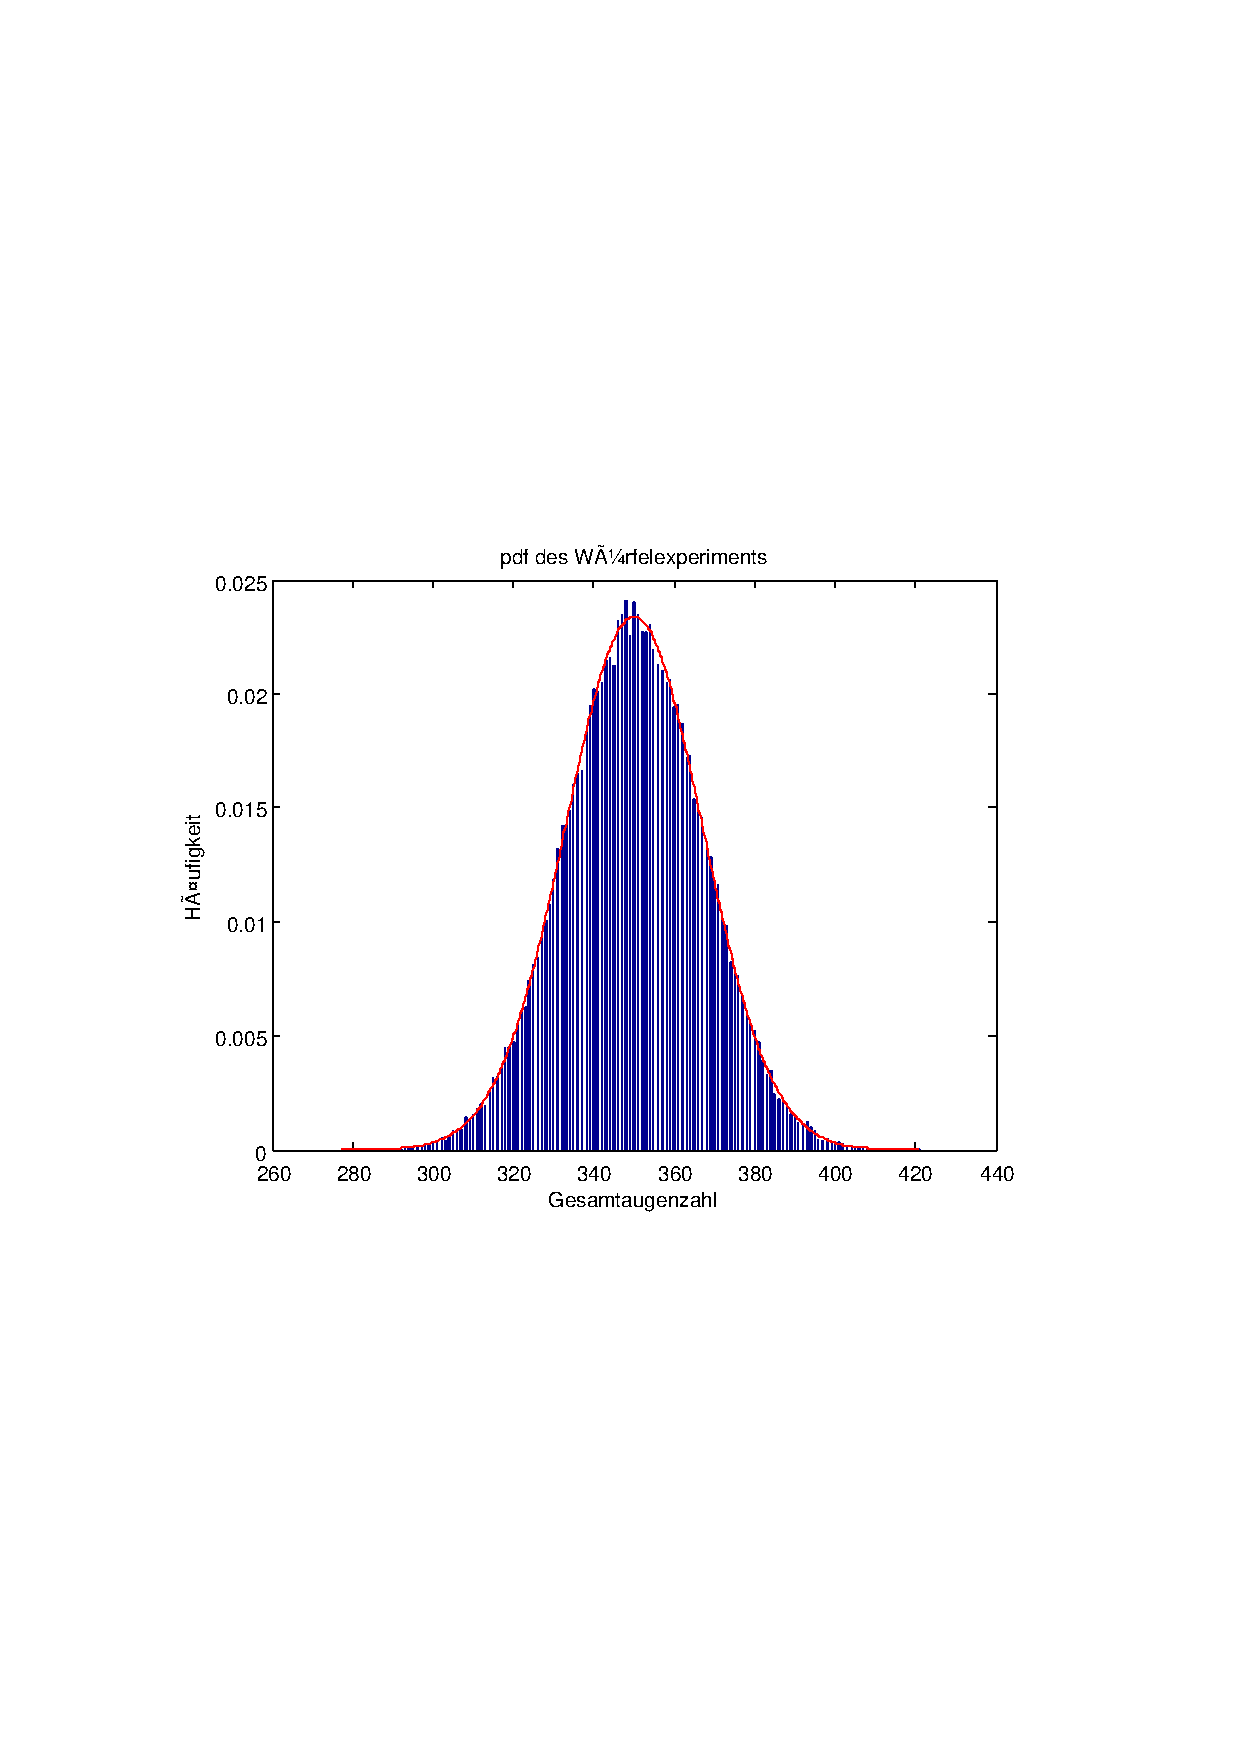
\includegraphics[scale=0.7, trim = 20mm 80mm 20mm 90mm, clip]{Bilder/A1_3_100}
                    \caption{Häufigkeitsverteilung: 100 Würfel}
                \end{figure}
        
            \end{minipage}
        
        \end{tabular}
        \end{center}


        \begin{figure}[H]
        \centering
            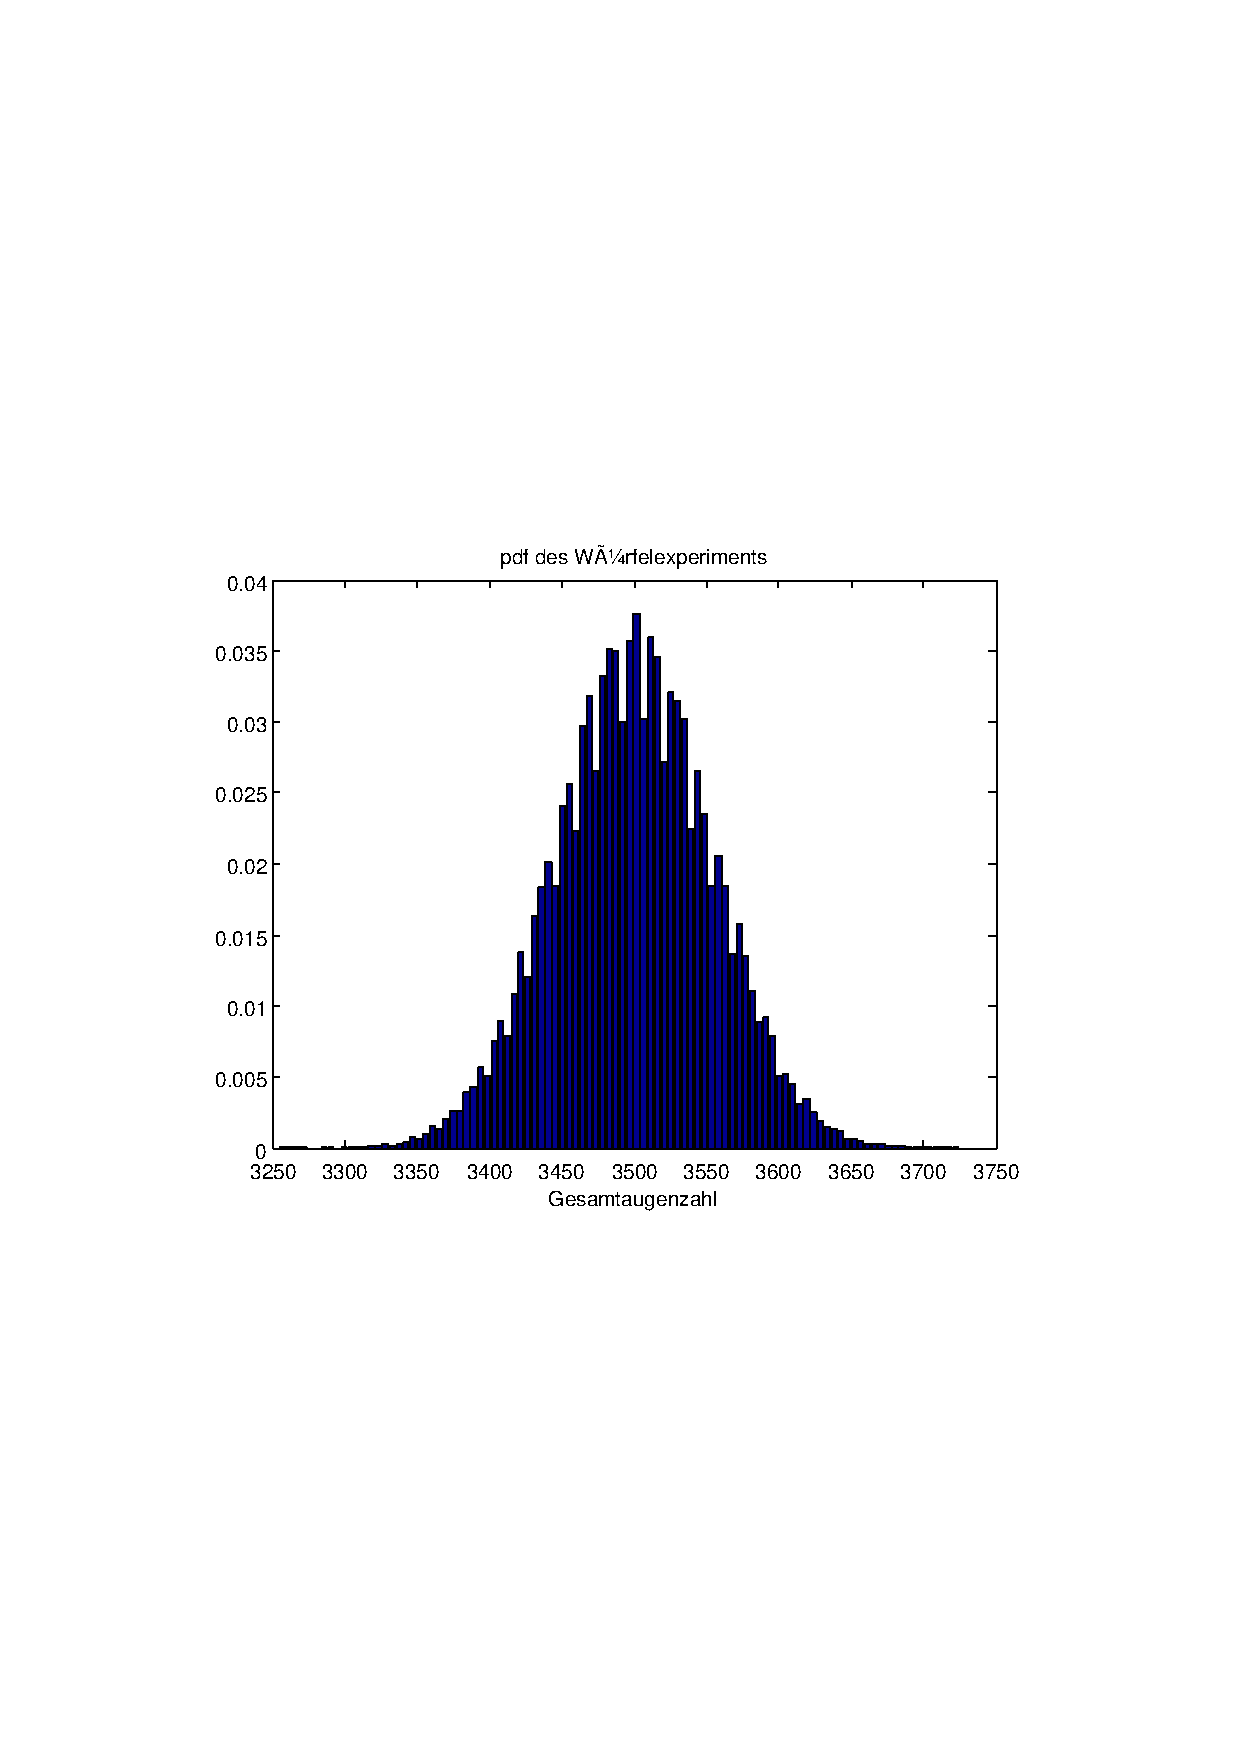
\includegraphics[scale=0.7, trim = 20mm 80mm 20mm 90mm, clip]{Bilder/A1_3_1000}
                \caption{Häufigkeitsverteilung: 1000 Würfel}
                \label{fig:A1_3_1000}
        \end{figure}
    


        \begin{quote}
            

            
            Es ist zu beobachten, dass sich, je mehr Würfel geworfen werden, die Verteilungsdichtefunktion der Gaußverteilung
            immmer weiter annähert.\\
            Die nicht ganz exakte form könnte man mit noch mehr Würfen weiter annähern.
            
            
            \lstinputlisting[
                caption={Matlab-script},
                label=lst:Matlab]
                {./Matlab/Aufgabe1_3.m}
            
        \end{quote}
        
        
    \end{quote}
    
\end{quote}

\section{Rauschbehafteter Übertragungskanal}
\begin{quote}
    
    
    \subsection{Labordurchführung}
    \begin{quote}
        Für diesen Versuch haben wir von dem Emona 101 ein pseudozufälliges, Binärsignal ohne Nulldurchgang erzeugen lassen, was
        ein zu übertragendes Signal simuliert hat. Dieses Signal haben wir, als Simulation einer Übertragung, mit einem
        mittelwertfreien Rauschen unterschiedlicher Amplituden addiert. Da es sich hierbei um weißes Rauschen hadelt,erwarten wir
        eine normal- bzw. Gaußverteilung. Für bessere visuelle Überprüfung plotten wir die Gauß- und zum Vergleich auch die
        Laplaceverteilung, über die normierte Häufigkeitsverteilung des Rauschens.\\
        Außerdem wird das Signal gedämpft werden, da zumindest ohmsche Verluste in den Leitungen auftreten werden.\\
        Um das Verhältniss von Signal und Rauschen zu vergleichen werden wir die SNRs (das logarythmierte Verhältniss von Signal
        und Rauschen) als ein Maß der Rauschbehaftetheit gegenüberstellen.
        
        %alle abweichungen des mittelwerts is dämpfung (rauschen mittelwertfrei)
        
    \end{quote}
    
    
    
    
    \subsection{Auswertung}
    
    Im Folgenden sollen aus bekanntem Sende- und Empfangssignal Dämpfung und Rauschcharakteristik
    eines Übertragungskanals bestimmt werden. Es darf angenommen werden, dass die Dämpfung des
    Systems sich lediglich linear auf die Amplitude des Sendesignals auswirkt.
    
    \begin{quote}
        
        \subsubsection{-20dB Rauschen}
        \begin{quote}
            
            
        \begin{center}
        \begin{tabular}{ll}
        
        \hspace{-16.5em}
            \begin{minipage}{0.6\textwidth}
                
                \begin{figure}[H]
                    \label{fig:rau20}
                    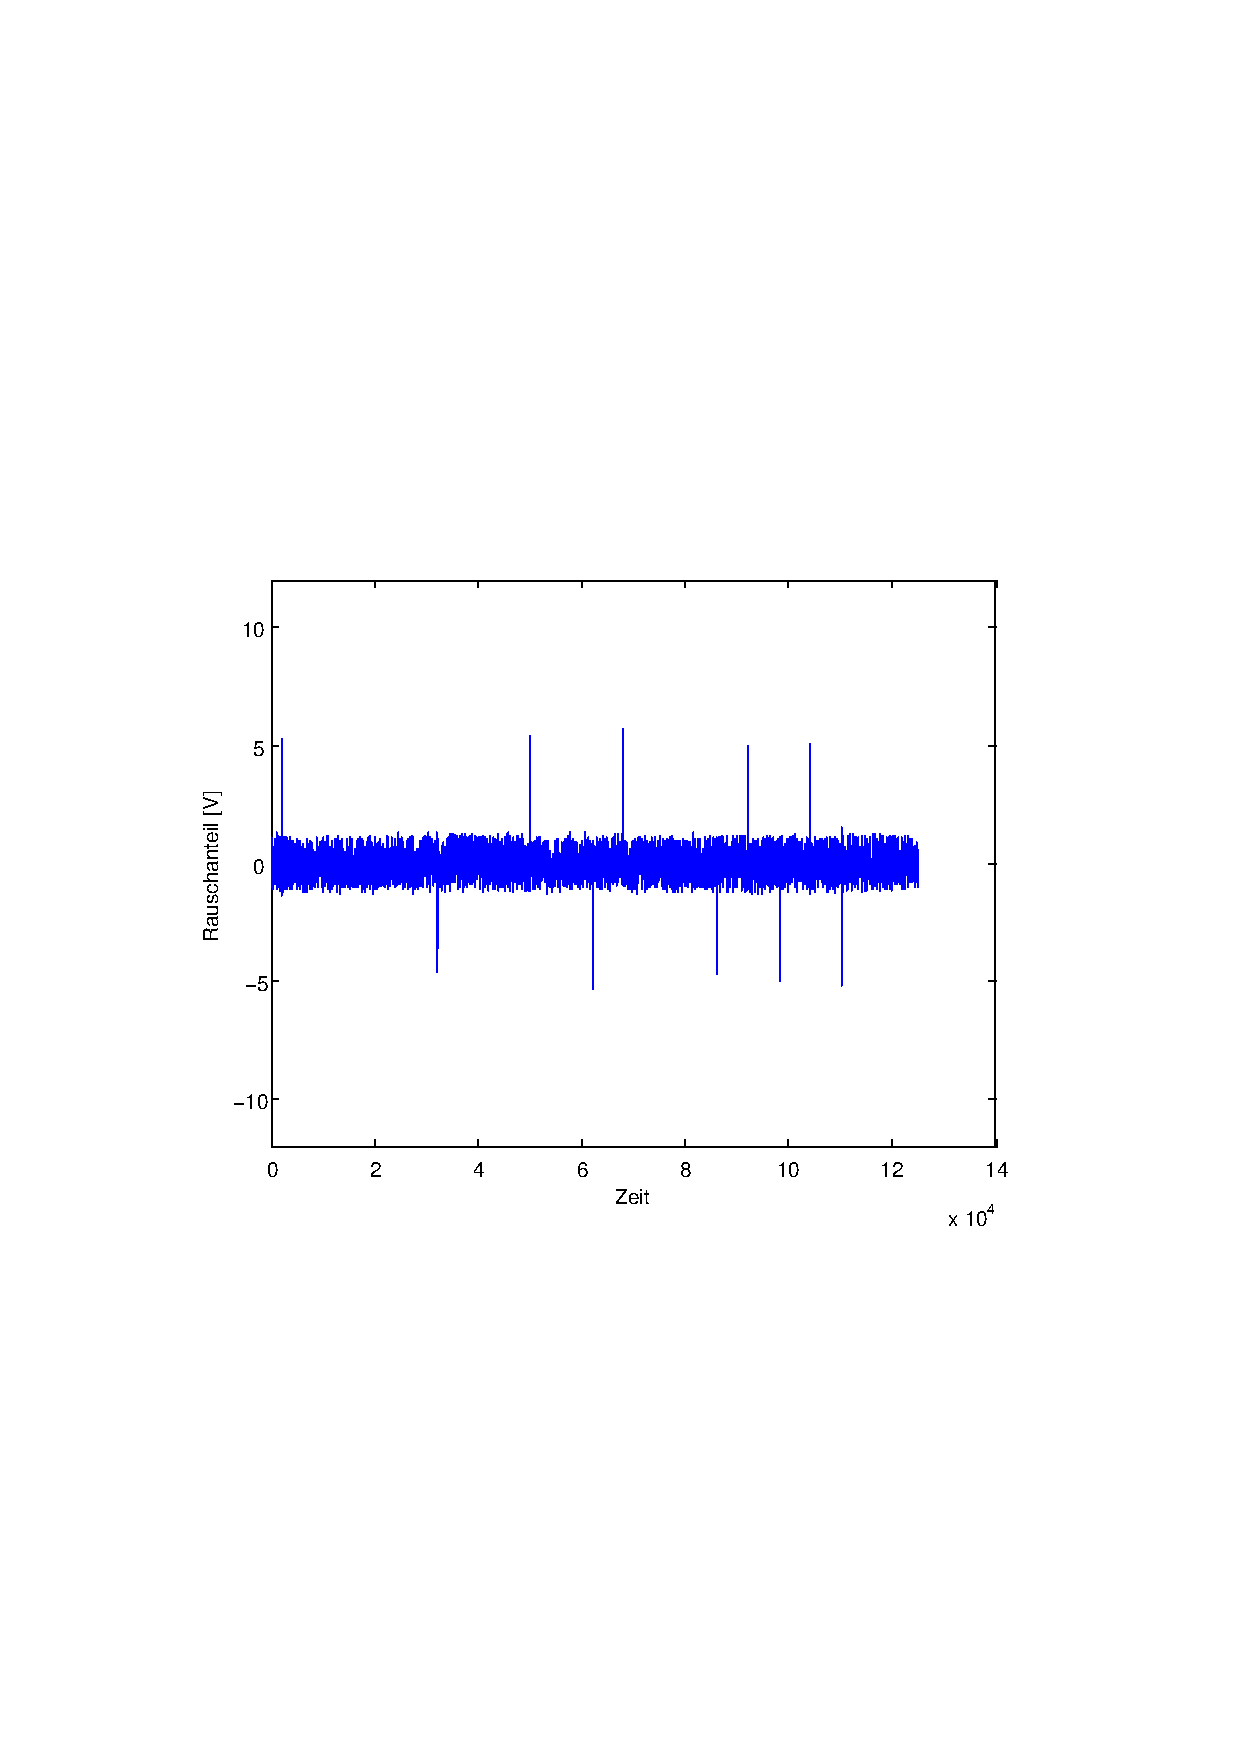
\includegraphics[scale=0.7, trim = 20mm 80mm 20mm 90mm, clip]{Bilder/rau20}
                    \caption{Rauschanteil des Signals mit -20dB Rauschen}
                \end{figure}
        
            \end{minipage}
        
            \begin{minipage}{0.6\textwidth}
                \begin{figure}[H]
                    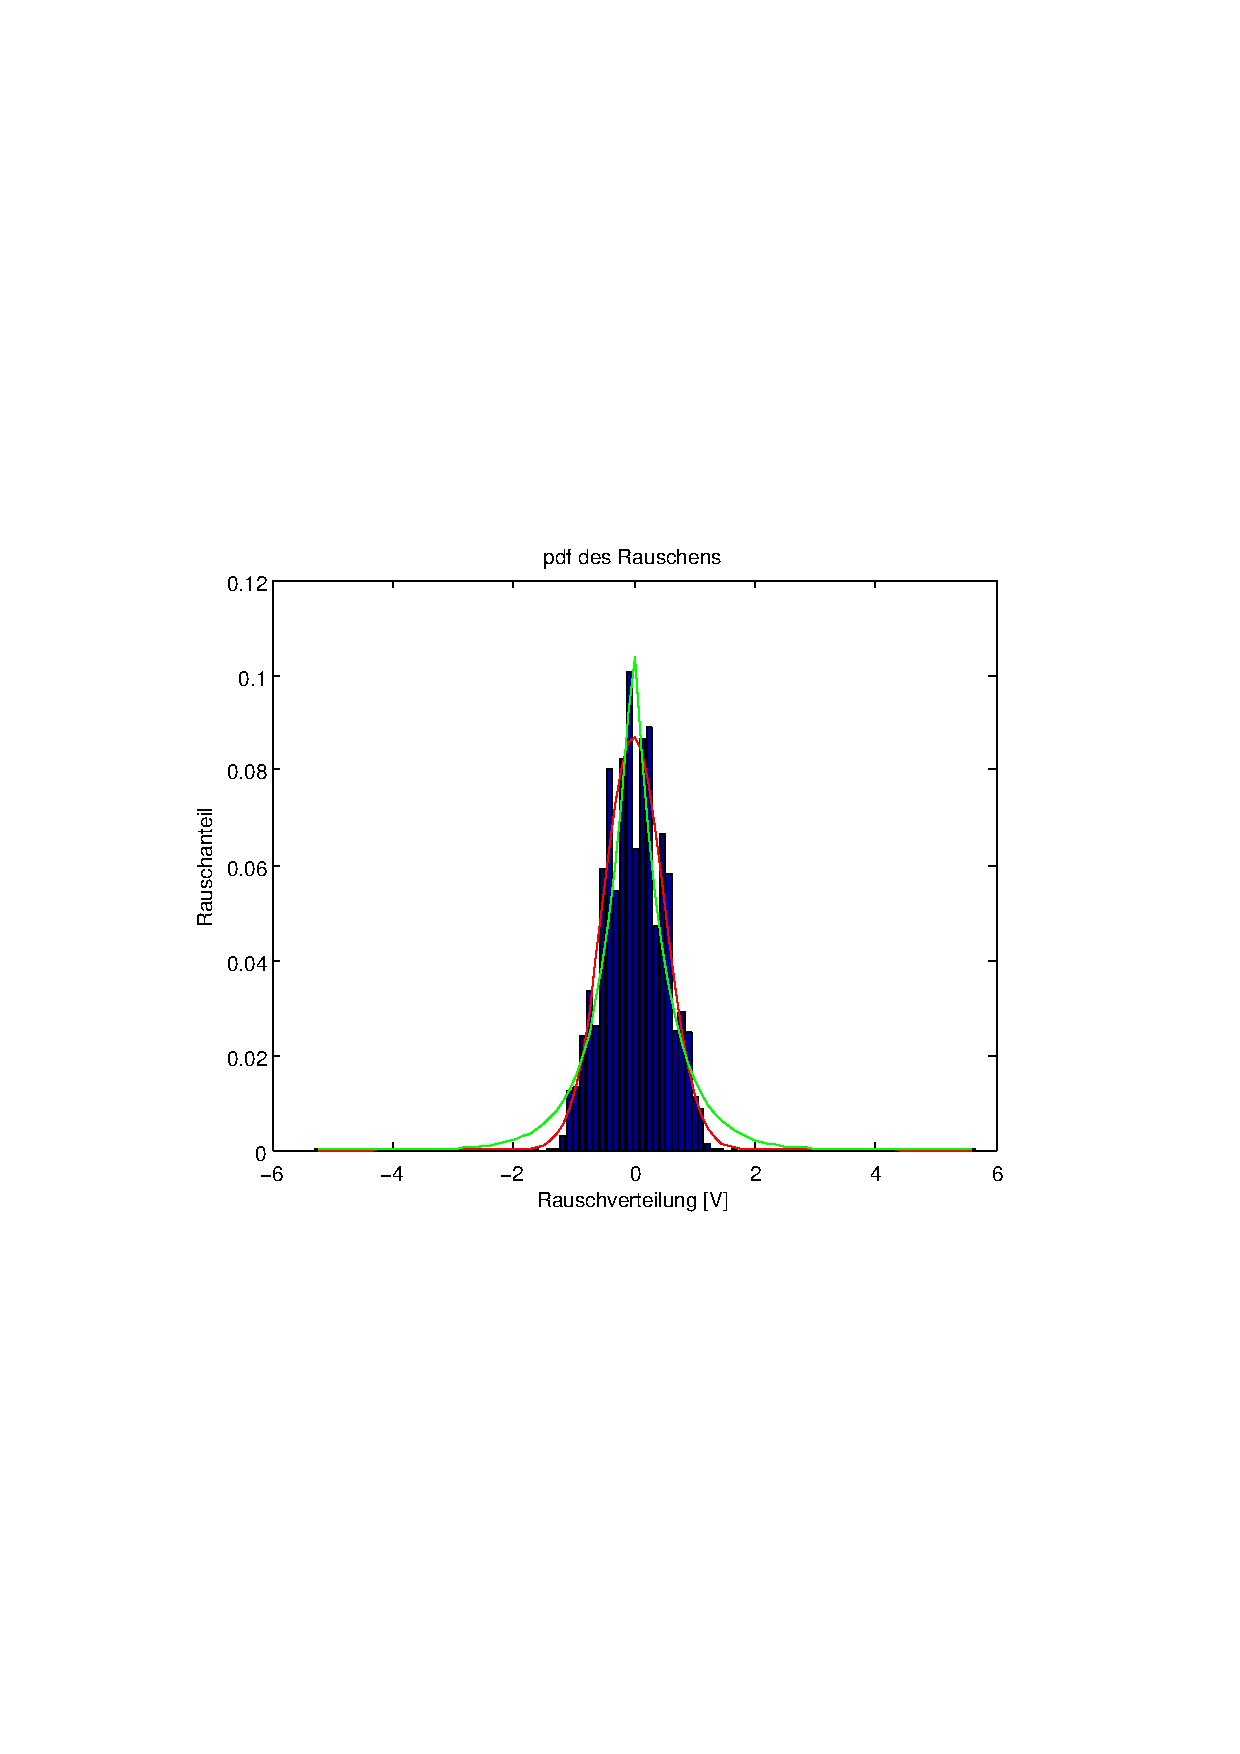
\includegraphics[scale=0.7, trim = 15mm 80mm 20mm 90mm, clip]{Bilder/hist20}
                    \caption{Häufigkeitsverteilung des Rauschens}
                    \label{fig:hist20}
                \end{figure}
            
            \end{minipage}
        
        \end{tabular}
        \end{center}
            
            \vspace{2em}
            
            \begin{equation*}
            \begin{split}
                 SNR = 17.7169
            \end{split}
            \end{equation*}
            
            Das Rauschen ist relativ gering mit ca. $ \pm2,5$ Volt. Es ist, wie in Abbildung \ref{fig:hist20}, eher Gauß- als
            Laplaceverteilt.
            
        \end{quote}
        
        
        \subsubsection{-6dB Rauchen}
        \begin{quote}
        \begin{center}
        \begin{tabular}{ll}
        
        \hspace{-16.5em}
            \begin{minipage}{0.6\textwidth}
                
                \begin{figure}[H]
                    \label{fig:funktion0alpha}
                    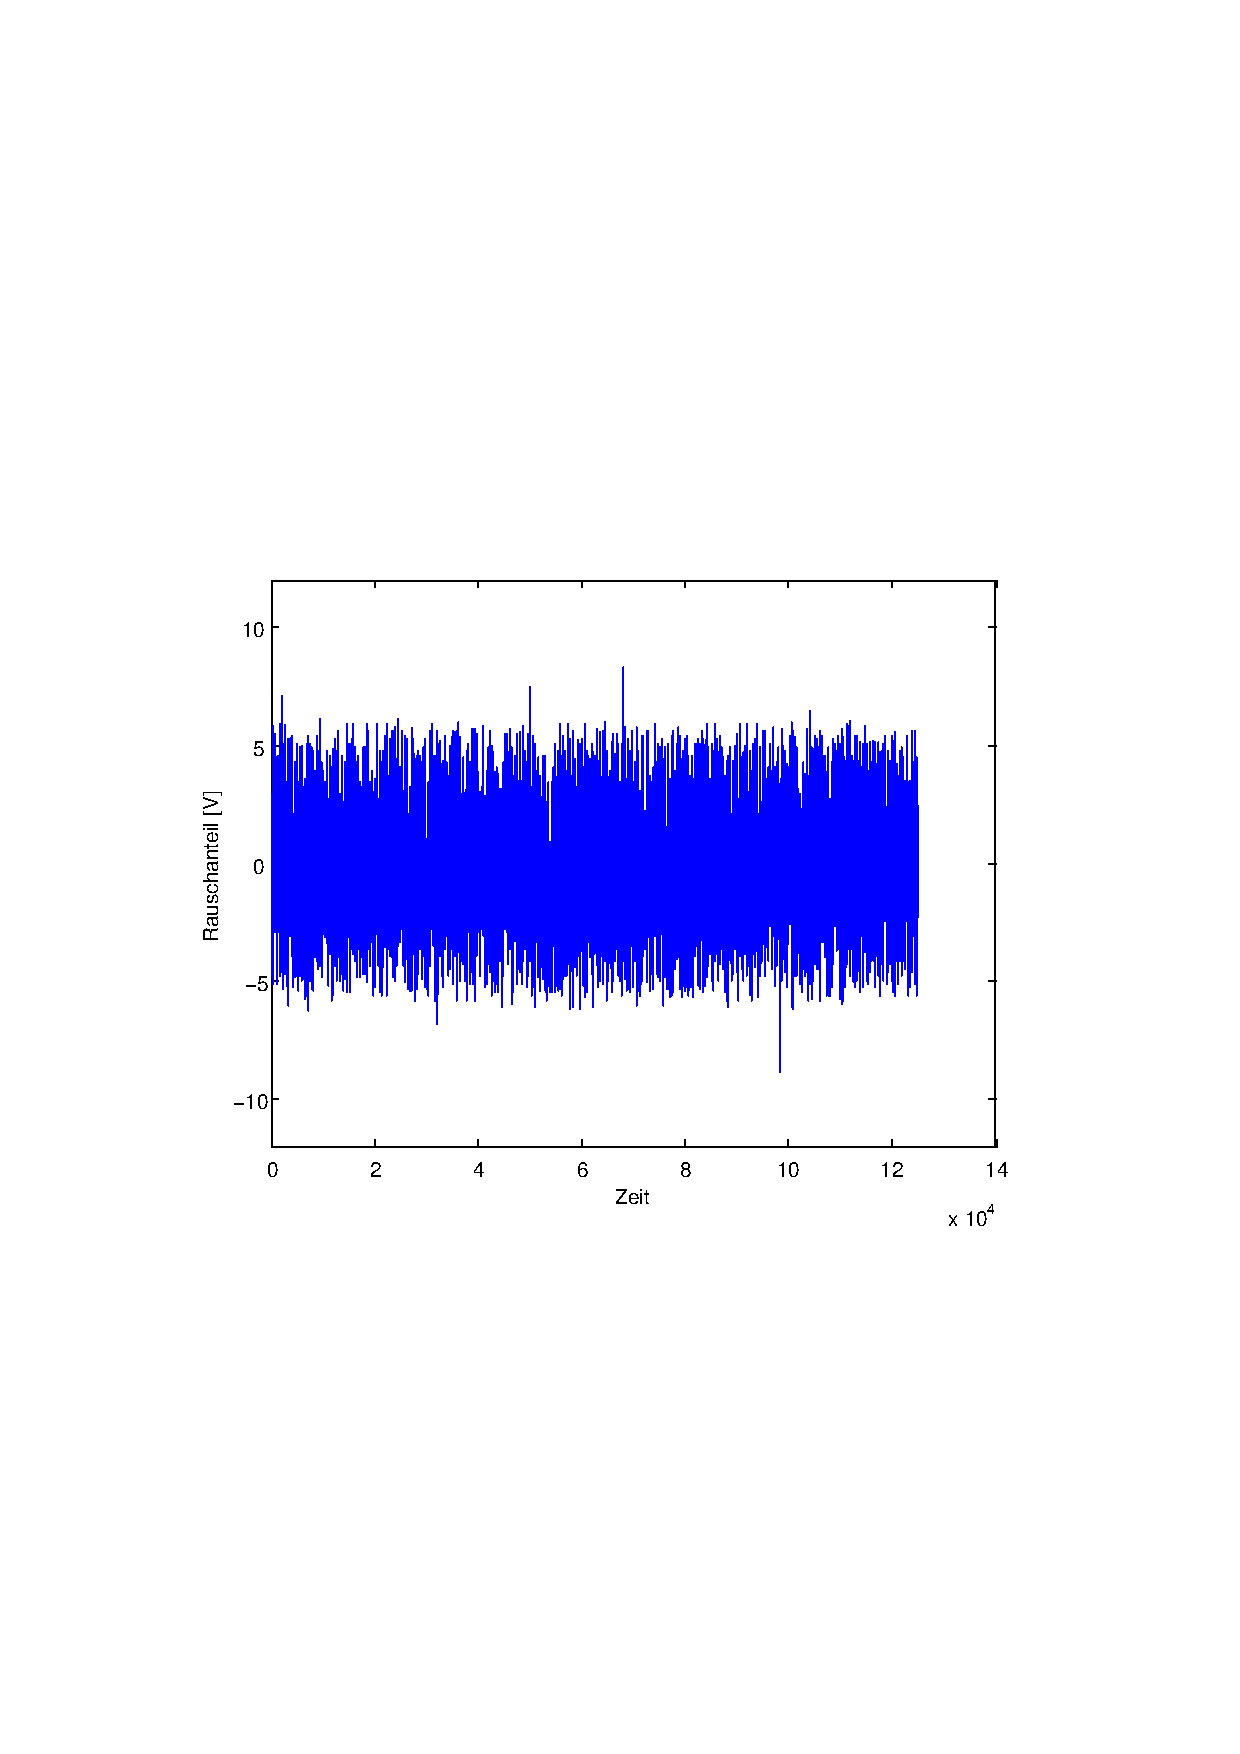
\includegraphics[scale=0.7, trim = 20mm 80mm 20mm 90mm, clip]{Bilder/rau6}
                    \caption{Rauschanteil des Signals mit -6dB Rauschen}
                \end{figure}
                
            \end{minipage}
            
            \begin{minipage}{0.6\textwidth}
                \begin{figure}[H]
                    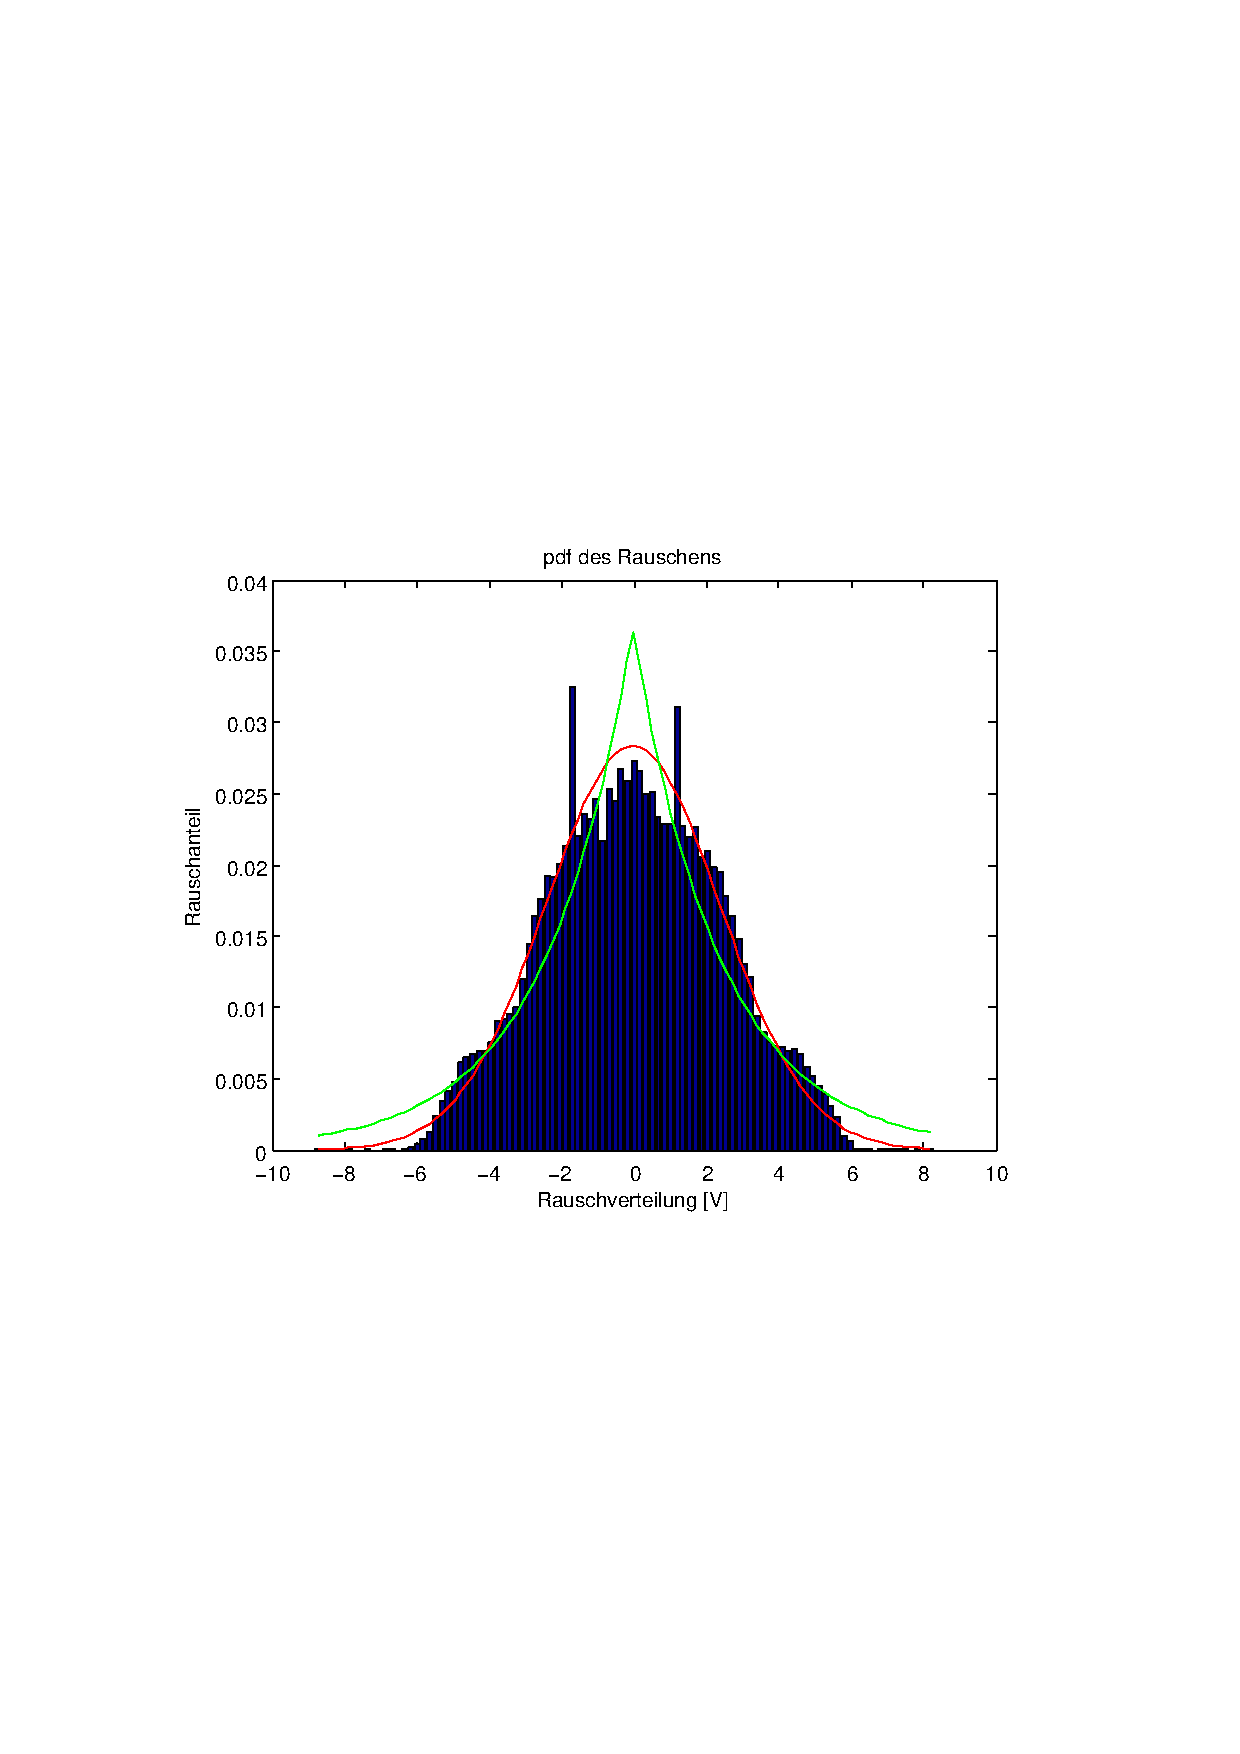
\includegraphics[scale=0.7, trim = 15mm 80mm 20mm 90mm, clip]{Bilder/hist6}
                    \caption{Häufigkeitsverteilung des Rauschens}
                    \label{fig:hist6}
                \end{figure}
                
            \end{minipage}
            
        \end{tabular}
        \end{center}
            
            \vspace{2em}
            \begin{equation*}
            \begin{split}
                 SNR = 5.5350
            \end{split}
            \end{equation*}
            
            Das Rauschen bei -6 dB ist mit ca. $\pm 4$ Volt schon deutlich größer. Die Verteilungsdichtefunktion \ref{fig:hist6}
            ist noch eindeutiger eine Gaußverteilung.\\
            Durch die größere Amplitude des Rauschens wird die Häufigkeitsverteilung natürlich breiter.
            
            
        \end{quote}
        
        \subsubsection{0dB Rauschen}
        \begin{quote}
        \begin{center}
        \begin{tabular}{ll}
        
        \hspace{-16.5em}
            \begin{minipage}{0.6\textwidth}
                
                \begin{figure}[H]
                    \label{fig:funktion0alpha}
                    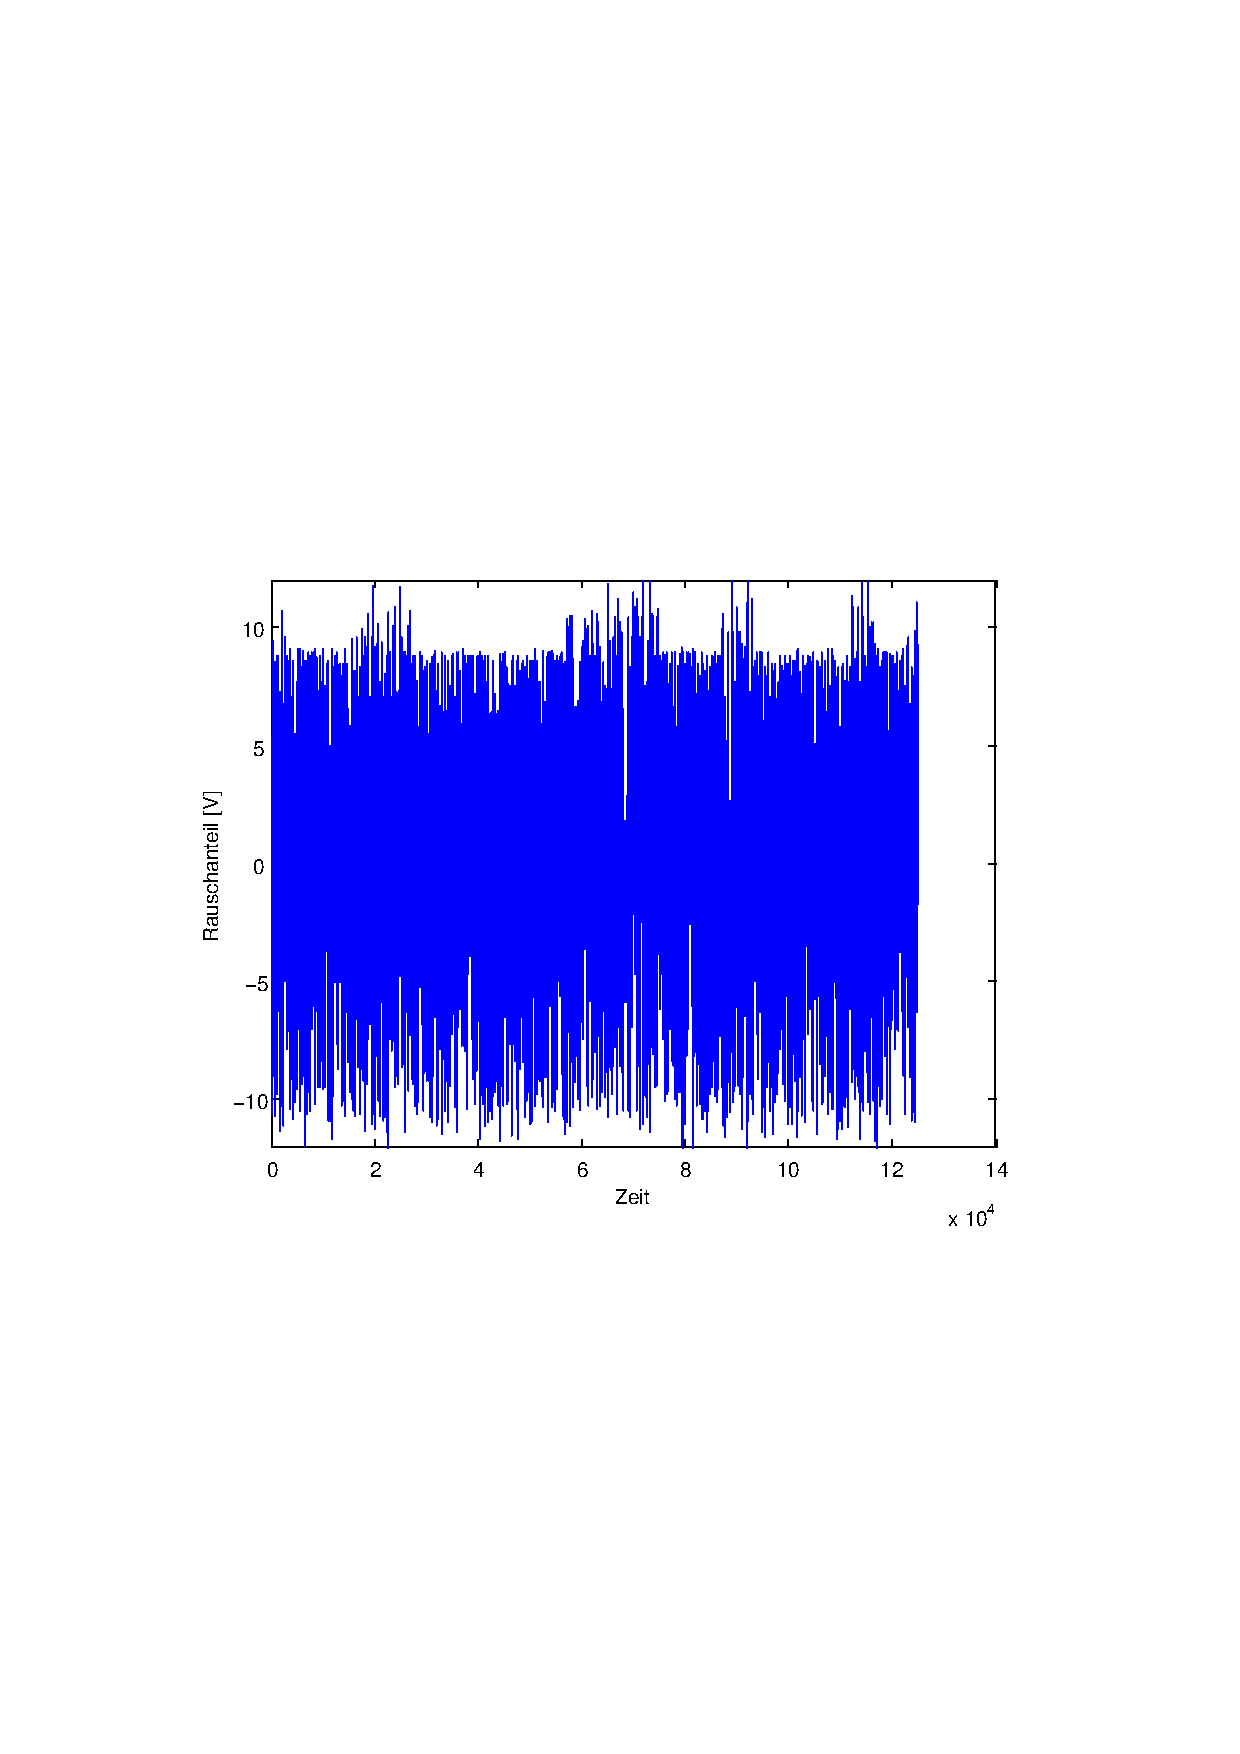
\includegraphics[scale=0.7, trim = 20mm 80mm 20mm 90mm, clip]{Bilder/rau0}
                    \caption{Rauschanteil des Signals mit 0dB Rauschen}
                \end{figure}
                
            \end{minipage}
            
            \begin{minipage}{0.6\textwidth}
                \begin{figure}[H]
                    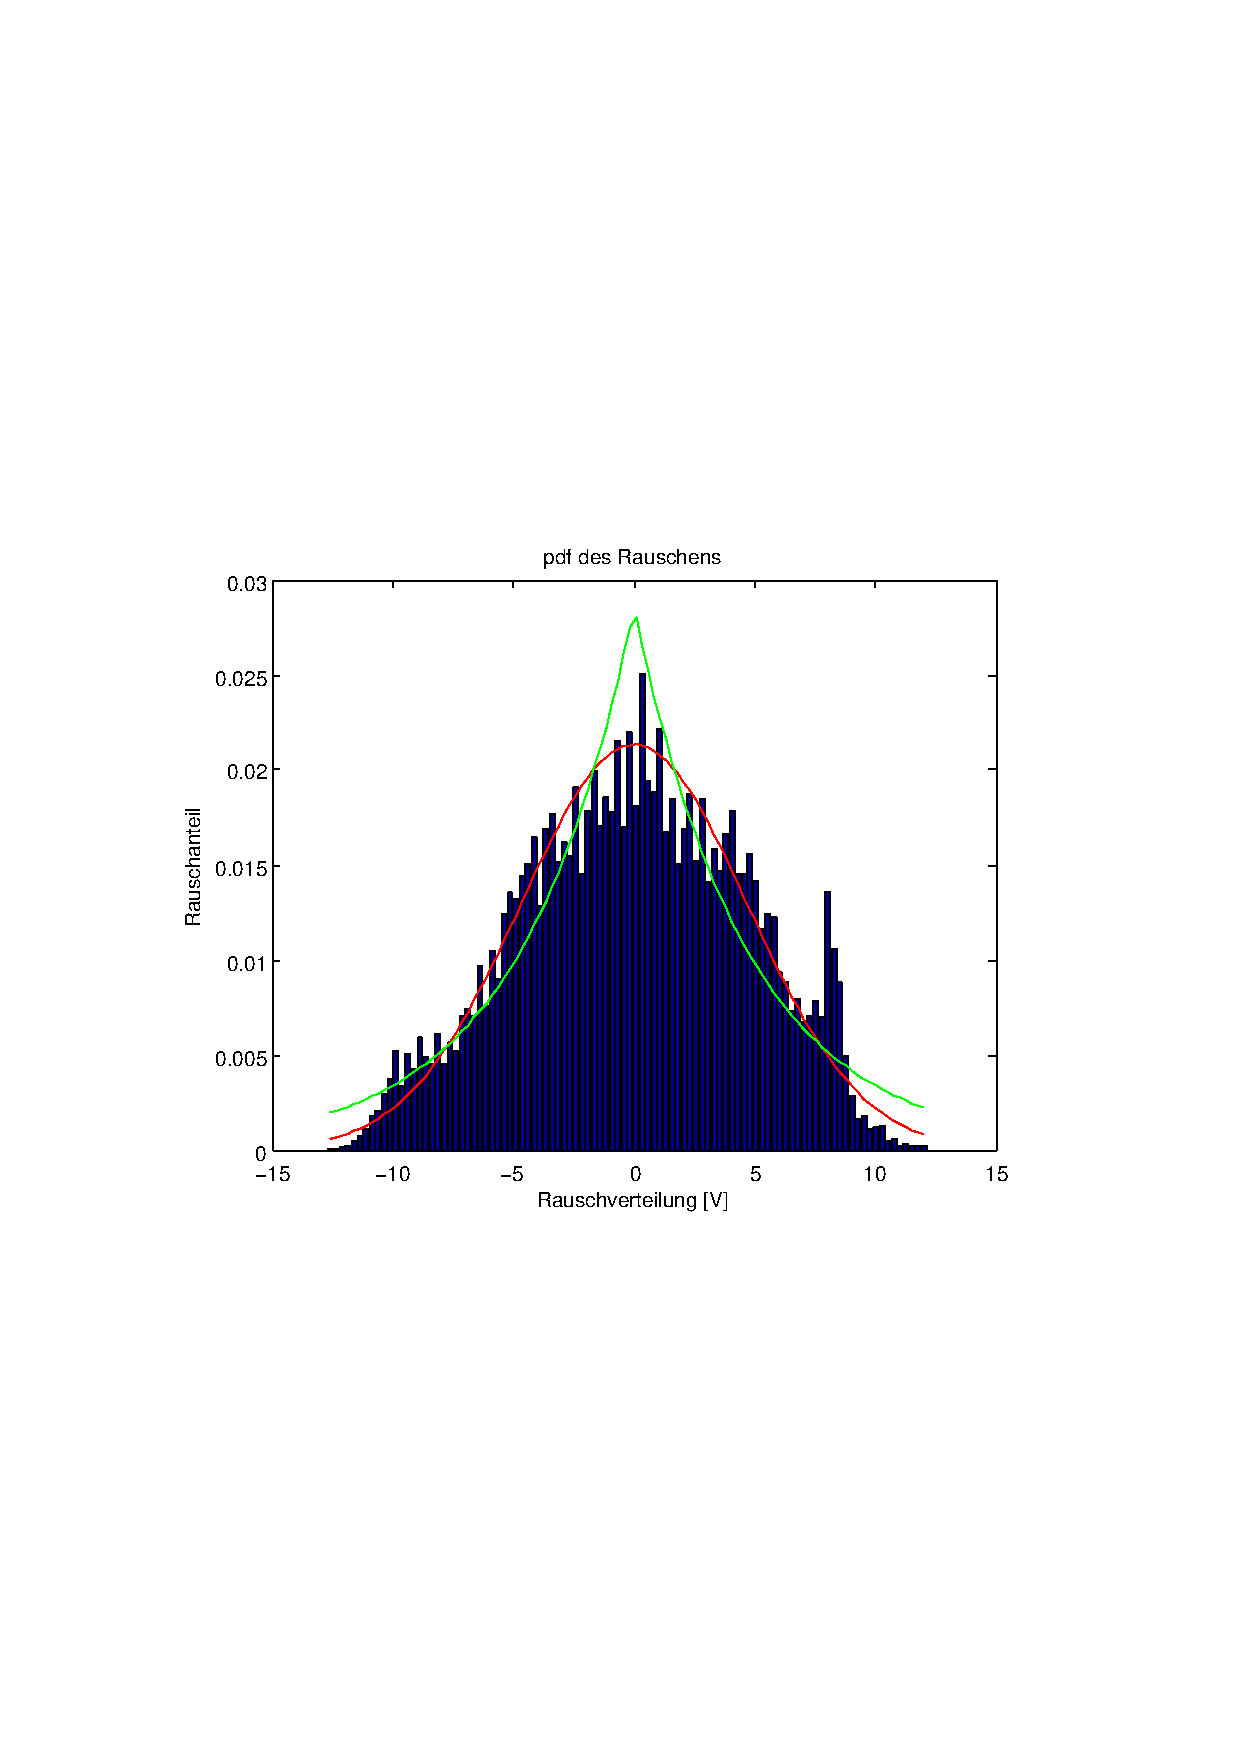
\includegraphics[scale=0.7, trim = 15mm 80mm 20mm 90mm, clip]{Bilder/hist0}
                    \caption{Häufigkeitsverteilung des Rauschens}
                    \label{fig:hist0}
                \end{figure}
                
            \end{minipage}
            
        \end{tabular}
        \end{center}
            
            \vspace{2em}
            
            \begin{equation*}
            \begin{split}
                 SNR = -1.9448
            \end{split}
            \end{equation*}
            
            Der Rauschanteil ist bei 0dB Rauschen mit ca. $\pm9$ Volt schon deutlich Größer als zuvor. Die Verteilung gleicht
            hier, bis auf einen kleinen Ausreißer, fast perfekt einer Gaußverteilung.
            
        \end{quote}
        
        \vspace{4em}
        
        Es ist deutlich zu erkennen, dass der Rauschanteil der Signale über die Messungen erheblich steigt.
        Beim der letzten Messung mit 0dB Rauschen ist der SNR sogar negariv; das Rauschen also größer als das eigentliche Signal.
        Die SNR Werte der drei Rauschsignale haben, wie erwartet, ca. den folgenden Linearen zusammenhang.
        
        \begin{equation*}
    	\begin{split}
    		\mathrm{SNR \ [dB]} = \mathrm{Rauchen \ [dB]} - 2 
    	\end{split}
        \end{equation*}
        
        \newpage
        \lstinputlisting[
            caption={Matlab-script},
            label=lst:Matlab]
            {./Matlab/Aufgabe2.m}
        
        \lstinputlisting[
            caption={Matlab-script},
            label=lst:Matlab]
            {./Matlab/SNR.m}
        
    \end{quote}
    
    
\end{quote}





% \begin{quote}
%     \lstinputlisting[
%         caption={Scilab-script},
%         label=lst:scilab]
%         {./Scilab/Motor.sce}
%         
% \end{quote}

%--------------------------------------------------------------------
%--------------------------------------------------------------------
% \begin{thebibliography}{999}
% 
% \bibitem{Boris}Boris Henckell: Ein Paar sachen geklaut.. ähhh inspirationen geholt
% \href{http://www.krachler.com/fileadmin/user_upload/arbeiten/Reglersynthese_Christian_Krachler.pdf}{Reglersynthese nach dem Frequenzkennlinienverfahren}, S16, S22, 08.05.2012
% 
% 
% %Name, Vorname.; evtl. Name2, Vorname2.: Titel des Dokumentes
% %oder Buches, Zeitschrift/Verlag/URL (Auflage, Erscheinungsort, -jahr), ggf. Seitenzahlen
% %\bibitem [Wiki10] {DigitaleMesskette2} \url{www.wikipedia.org}, Zugriff 22.03.2010
% \end{thebibliography}


\end{document}
